\documentclass{article}
\usepackage{fancyhdr}
\usepackage{tikz}
\usepackage{xcolor}
\usepackage{ifthenx}
\usetikzlibrary{calc}
\usetikzlibrary{arrows.meta}% 箭头库
\usetikzlibrary{shapes}
%%%%%%%%%%%%%%%%%%%%%写个链表样式%%%%%%%%
\tikzstyle{ptr}  = [draw, -{Stealth[scale=1.0]}, black]
\tikzstyle{head} = [rectangle, draw=none, text height=3mm, text width=3mm,
                    text centered, node distance=3cm, inner sep=0pt]
\tikzstyle{data} = [rectangle split, rectangle split parts=2, draw,
                    text centered, minimum height=3em]
\newcommand{\data}{
  data \nodepart{second}
  \phantom{\texttt{NULL}}
}
%%%%%%%%%%%%%%%%%%%%%%%%%%%%%%%%%%%%%%
\pagestyle{fancy}
\setlength{\headheight}{35pt}
\lhead{Datenstrukturen \& Algorithmen\\Sommersemester2020\\Übungsblatt 1}
\chead{}
% bfseries
\rhead{Ciheng Zhang(3472321)\\Yao He(3487882)\\YuchanBian(3496226)}
\cfoot{\thepage}
\renewcommand{\headrulewidth}{0.4pt}

\begin{document}
\begin{titlepage}
    \title{\Huge \textbf{Datenstrukturen \& Algorithmen Gruppeübung\\Gruppe 10} }
    \author{\LARGE \textsl{Ciheng Zhang (3472321) zch3183505@gmail.com}\\\LARGE \textsl{Yao He (3487882) st168323@stud.uni-stuttgart.de}\\\LARGE \textsl{Yuchan Bian (3496226) st170182@stud.uni-stuttgart.de} \\[200pt]}
    \date{\today}
    \maketitle
    \thispagestyle{empty}
\end{titlepage}
\newpage
\section{Aufgabe 1}
Sequenzielle Suche für a:\\
\begin{tikzpicture}
    [transition/.style={rectangle, draw=black!75 ,thick, minimum size=7mm}]
    \foreach \x/\y/\z in {13/0.5/red,23/1.2/red,47/1.9/red,48/2.6/red,68/3.3/red,12/4/red,69/4.7/gray,73/5.4/gray,81/6.1/gray,83/6.8/gray,84/7.5/gray,85/8.2/gray,87/8.9/gray,90/9.6/gray,94/10.3/gray}{
        \node(\x)[transition,fill=\z!20,] at (\y,0) {\x};
    }\\
\end{tikzpicture}\\
Das suchen Program sucht von die erste Element in die Array, Wenn diese Element it gleich wie die gesuchtes Element, die Program return die element und die Index von diese Element.Wie die Bild
die rote Element ist gesucht, Gray Element ist nicht gesucht. D.h. die Program hat 6 mal Loop und dann bekommt mann die result.
\\Sequenzielle Suche für b:\\
\begin{tikzpicture}
    [transition/.style={rectangle, draw=black!75 ,thick, minimum size=7mm}]
    \foreach \x/\y/\z in {12/0.5/red,13/1.2/red,23/1.9/red,47/2.6/red,48/3.3/red,68/4/red,69/4.7/gray,73/5.4/gray,81/6.1/gray,83/6.8/gray,84/7.5/gray,85/8.2/gray,87/8.9/gray,90/9.6/gray,94/10.3/gray}{
        \node(\x)[transition,fill=\z!20,] at (\y,0) {\x};
    }\\
\end{tikzpicture}\\
Änhlich Wie die letzen Methode. Durch Sequenzielle Suche braucht mann 5 mal Loop, um die Zahl 68 zu suchen\\
\\
\\
Binäre Suche für a:\\
Mann kann Binäre suchen für Aufgabe a nicht benutzen. Denn die Folgen ist nicht sortiert. Wenn mann möchte Binäre Suche für ein Folgen benutzen, muss die Folgen gesortirt wird.
\\
Binäre Suche für b:\\
\begin{tikzpicture}
    [transition/.style={rectangle, draw=black!75 ,thick, minimum size=7mm}]
    \foreach \x/\y/\z/\m in {12/0.5/gray/0,13/1.2/gray/1,23/1.9/gray/2,47/2.6/gray/3,48/3.3/gray/4,68/4/gray/5,69/4.7/gray/6,73/5.4/gray/7,81/6.1/gray/8,83/6.8/gray/9,84/7.5/gray/10,85/8.2/gray/11,87/8.9/gray/12,90/9.6/gray/13,94/10.3/gray/14}{
        \node(\x)[transition,fill=\z!20,] at (\y,0) {\x};
        \node(blank\x)[transition] at (\y,-0.7) {\ifthenelse{\m = 7}{m}{\ifthenelse{\m=0}{u}{\ifthenelse{\m=14}{o}{ }} }};  
    }\\
\end{tikzpicture}\\
zuerst man bekommt die Middle Zahl in die ganze Folgen und zeichen es m und bekommt mann die wert.
dann 68<73. Man macht ein neue Folgen von u bis m\\
\begin{tikzpicture}
    [transition/.style={rectangle, draw=black!75 ,thick, minimum size=7mm}]
    \foreach \x/\y/\z/\m in {12/0.5/gray/0,13/1.2/gray/1,23/1.9/gray/2,47/2.6/gray/3,48/3.3/gray/4,68/4/gray/5,69/4.7/gray/6,73/5.4/gray/7}{
        \node(\x)[transition,fill=\z!20,] at (\y,0) {\x};
        \node(blank\x)[transition] at (\y,-0.7) {\ifthenelse{\m = 3}{m}{\ifthenelse{\m=0}{u}{\ifthenelse{\m=7}{o}{ }} }};  
    }\\
\end{tikzpicture}\\
Wieder Machen die letzen Methode. Zahl m ist 47. gesucht Zahl 68 ist großer als 48. dann Wieder ein neue Folgen von m bis o Machen.
\\
\begin{tikzpicture}
    [transition/.style={rectangle, draw=black!75 ,thick, minimum size=7mm}]
    \foreach \x/\y/\z/\m in {47/2.6/gray/3,48/3.3/gray/4,68/4/red/5,69/4.7/gray/6,73/5.4/gray/7}{
        \node(\x)[transition,fill=\z!20,] at (\y,0) {\x};
        \node(blank\x)[transition] at (\y,-0.7) {\ifthenelse{\m = 5}{m}{\ifthenelse{\m=3}{u}{\ifthenelse{\m=7}{o}{ }} }};  
    }\\
\end{tikzpicture}\\
Dann bekommt man die m Wert ist 68 gleich wie gesucht Element.Und man bekommt die gesucht Wert mit 3 mal Loop. Es ist schneller als die Sequenzielle Suche.Aus diese Grund
benutzen mann die Binäre Suche für Aufgabe b\\

\section{Aufgabe 2}
Lösung im beigefügten Eclipse-Project

\section{Aufgabe 3}
\subsection*{(a)}
\def\scaleratio{0.8}
%%%%%%%%%%%%%%%%这里开始画弱智链表结构%%%%%%%%%%%%%%%%%%%

\begin{figure}[!h]
  \centering
  \begin{tikzpicture}[node distance=1.25cm, auto, scale=\scaleratio,
    every node/.style={scale=\scaleratio}]
    \node[head, label=below:phead] (head) {};

    \node[data, right of=head] (A) {6};
    \node[right of=A,node distance=0.25cm] (a1){};
    \node[data, right of=A] (B) {13};
    \node[right of=B,node distance=0.25cm] (a2){};
    \node[data, right of=B] (C) {8};
    \node[right of=C,node distance=0.25cm] (a3){};
    \node[data, right of=C] (D) {5};
    \node[right of=D,node distance=0.25cm] (a4){};

    \node[data, right of=D] (E) {14};
    \node[right of=E,node distance=0.25cm] (a5){};
    \node[data, right of=E] (F) {33};
    \node[right of=F,node distance=0.25cm] (a6){};
    \node[data, right of=F] (G) {95};
    \node[right of=G,node distance=0.25cm] (a7){};
    \node[data, right of=G] (H) {73};
    \node[right of=H,node distance=0.25cm] (a8){};
    \node[data, right of=H] (I) {55};
    \node[right of=I,node distance=0.25cm] (a9){};
    \node[data, right of=I] (J) {64};
    \node[right of=I,node distance=0.25cm] (a10){};
    \node[data, right of=J] (last) {\nodepart{second} \texttt{NULL}};
    \node[right of=last,node distance=0.25cm] (a11){};
    
    

    \draw[fill] (head.center) circle (0.05);

    \path[ptr] (head.center) --++(right:5mm) |- (A.text west);
    \draw[fill] ($(A.south)!0.5!(A.text split)$) circle (0.05);
    \draw[ptr] ($(A.south)!0.5!(A.text split)$) --++(right:5mm) |- (B.text west);
    \draw[fill] ($(B.south)!0.5!(B.text split)$) circle (0.05);
    \draw[ptr] ($(B.south)!0.5!(B.text split)$) --++(right:5mm) |- (C.text west);
    \draw[fill] ($(C.south)!0.5!(C.text split)$) circle (0.05);
    \draw[ptr] ($(C.south)!0.5!(C.text split)$) --++(right:5mm) |- (D.text west);
    \draw[fill] ($(D.south)!0.5!(D.text split)$) circle (0.05);
    \draw[ptr] ($(D.south)!0.5!(D.text split)$) --++(right:5mm) |- (E.text west);
    
    \draw[fill] ($(E.south)!0.5!(E.text split)$) circle (0.05);
    \draw[ptr] ($(E.south)!0.5!(E.text split)$) --++(right:5mm) |- (F.text west);
    \draw[fill] ($(F.south)!0.5!(F.text split)$) circle (0.05);
    \draw[ptr] ($(F.south)!0.5!(F.text split)$) --++(right:5mm) |- (G.text west);
    \draw[fill] ($(G.south)!0.5!(G.text split)$) circle (0.05);
    \draw[ptr] ($(G.south)!0.5!(G.text split)$) --++(right:5mm) |- (H.text west);
    \draw[fill] ($(H.south)!0.5!(H.text split)$) circle (0.05);
    \draw[ptr] ($(H.south)!0.5!(H.text split)$) --++(right:5mm) |- (I.text west);
    \draw[fill] ($(I.south)!0.5!(I.text split)$) circle (0.05);
    \draw[ptr] ($(I.south)!0.5!(I.text split)$) --++(right:5mm) |- (J.text west);

    \draw[fill] ($(J.south)!0.5!(J.text split)$) circle (0.05);
    \draw[ptr] ($(J.south)!0.5!(J.text split)$) --++(right:5mm) |- (last.text west);
  \end{tikzpicture}
\end{figure}
%%%%%%%%%%链表结构结束%%%%%%%%%%%%%%%%%%%%%%%%%%%%%%

%%%%%%%%%%%%%%%%这里开始画弱智链表结构%%%%%%%%%%%%%%%%%%%

\begin{figure}[!h]
    \centering
    \begin{tikzpicture}[node distance=1.25cm, auto, scale=\scaleratio,
      every node/.style={scale=\scaleratio}]
      \node[head, label=below:phead] (head) {};
  
      \node[data, right of=head] (A) {6};
      \node[right of=A,node distance=0.25cm] (a1){};
      \node[data, right of=A] (B) {8};
      \node[right of=B,node distance=0.25cm] (a2){};
      \node[data, right of=B] (C) {5};
      \node[right of=C,node distance=0.25cm] (a3){};
      \node[data, right of=C] (D) {13};
      \node[right of=D,node distance=0.25cm] (a4){};
  
      \node[data, right of=D] (E) {14};
      \node[right of=E,node distance=0.25cm] (a5){};
      \node[data, right of=E] (F) {33};
      \node[right of=F,node distance=0.25cm] (a6){};
      \node[data, right of=F] (G) {73};
      \node[right of=G,node distance=0.25cm] (a7){};
      \node[data, right of=G] (H) {55};
      \node[right of=H,node distance=0.25cm] (a8){};
      \node[data, right of=H] (I) {64};
      \node[right of=I,node distance=0.25cm] (a9){};
      \node[data, right of=I] (J) {95};
      \node[right of=I,node distance=0.25cm] (a10){};
      \node[data, right of=J] (last) {\nodepart{second} \texttt{NULL}};
      \node[right of=last,node distance=0.25cm] (a11){};
      
      
  
      \draw[fill] (head.center) circle (0.05);
  
      \path[ptr] (head.center) --++(right:5mm) |- (A.text west);
      \draw[fill] ($(A.south)!0.5!(A.text split)$) circle (0.05);
      \draw[ptr] ($(A.south)!0.5!(A.text split)$) --++(right:5mm) |- (B.text west);
      \draw[fill] ($(B.south)!0.5!(B.text split)$) circle (0.05);
      \draw[ptr] ($(B.south)!0.5!(B.text split)$) --++(right:5mm) |- (C.text west);
      \draw[fill] ($(C.south)!0.5!(C.text split)$) circle (0.05);
      \draw[ptr] ($(C.south)!0.5!(C.text split)$) --++(right:5mm) |- (D.text west);
      \draw[fill] ($(D.south)!0.5!(D.text split)$) circle (0.05);
      \draw[ptr] ($(D.south)!0.5!(D.text split)$) --++(right:5mm) |- (E.text west);
      
      \draw[fill] ($(E.south)!0.5!(E.text split)$) circle (0.05);
      \draw[ptr] ($(E.south)!0.5!(E.text split)$) --++(right:5mm) |- (F.text west);
      \draw[fill] ($(F.south)!0.5!(F.text split)$) circle (0.05);
      \draw[ptr] ($(F.south)!0.5!(F.text split)$) --++(right:5mm) |- (G.text west);
      \draw[fill] ($(G.south)!0.5!(G.text split)$) circle (0.05);
      \draw[ptr] ($(G.south)!0.5!(G.text split)$) --++(right:5mm) |- (H.text west);
      \draw[fill] ($(H.south)!0.5!(H.text split)$) circle (0.05);
      \draw[ptr] ($(H.south)!0.5!(H.text split)$) --++(right:5mm) |- (I.text west);
      \draw[fill] ($(I.south)!0.5!(I.text split)$) circle (0.05);
      \draw[ptr] ($(I.south)!0.5!(I.text split)$) --++(right:5mm) |- (J.text west);
  
      \draw[fill] ($(J.south)!0.5!(J.text split)$) circle (0.05);
      \draw[ptr] ($(J.south)!0.5!(J.text split)$) --++(right:5mm) |- (last.text west);
    \end{tikzpicture}
  \end{figure}
  %%%%%%%%%%链表结构结束%%%%%%%%%%%%%%%%%%%%%%%%%%%%%%

  %%%%%%%%%%%%%%%%这里开始画弱智链表结构%%%%%%%%%%%%%%%%%%%

\begin{figure}[!h]
    \centering
    \begin{tikzpicture}[node distance=1.25cm, auto, scale=\scaleratio,
      every node/.style={scale=\scaleratio}]
      \node[head, label=below:phead] (head) {};
  
      \node[data, right of=head] (A) {6};
      \node[right of=A,node distance=0.25cm] (a1){};
      \node[data, right of=A] (B) {5};
      \node[right of=B,node distance=0.25cm] (a2){};
      \node[data, right of=B] (C) {8};
      \node[right of=C,node distance=0.25cm] (a3){};
      \node[data, right of=C] (D) {13};
      \node[right of=D,node distance=0.25cm] (a4){};
  
      \node[data, right of=D] (E) {14};
      \node[right of=E,node distance=0.25cm] (a5){};
      \node[data, right of=E] (F) {33};
      \node[right of=F,node distance=0.25cm] (a6){};
      \node[data, right of=F] (G) {55};
      \node[right of=G,node distance=0.25cm] (a7){};
      \node[data, right of=G] (H) {64};
      \node[right of=H,node distance=0.25cm] (a8){};
      \node[data, right of=H] (I) {73};
      \node[right of=I,node distance=0.25cm] (a9){};
      \node[data, right of=I] (J) {95};
      \node[right of=I,node distance=0.25cm] (a10){};
      \node[data, right of=J] (last) {\nodepart{second} \texttt{NULL}};
      \node[right of=last,node distance=0.25cm] (a11){};
      
      
  
      \draw[fill] (head.center) circle (0.05);
  
      \path[ptr] (head.center) --++(right:5mm) |- (A.text west);
      \draw[fill] ($(A.south)!0.5!(A.text split)$) circle (0.05);
      \draw[ptr] ($(A.south)!0.5!(A.text split)$) --++(right:5mm) |- (B.text west);
      \draw[fill] ($(B.south)!0.5!(B.text split)$) circle (0.05);
      \draw[ptr] ($(B.south)!0.5!(B.text split)$) --++(right:5mm) |- (C.text west);
      \draw[fill] ($(C.south)!0.5!(C.text split)$) circle (0.05);
      \draw[ptr] ($(C.south)!0.5!(C.text split)$) --++(right:5mm) |- (D.text west);
      \draw[fill] ($(D.south)!0.5!(D.text split)$) circle (0.05);
      \draw[ptr] ($(D.south)!0.5!(D.text split)$) --++(right:5mm) |- (E.text west);
      
      \draw[fill] ($(E.south)!0.5!(E.text split)$) circle (0.05);
      \draw[ptr] ($(E.south)!0.5!(E.text split)$) --++(right:5mm) |- (F.text west);
      \draw[fill] ($(F.south)!0.5!(F.text split)$) circle (0.05);
      \draw[ptr] ($(F.south)!0.5!(F.text split)$) --++(right:5mm) |- (G.text west);
      \draw[fill] ($(G.south)!0.5!(G.text split)$) circle (0.05);
      \draw[ptr] ($(G.south)!0.5!(G.text split)$) --++(right:5mm) |- (H.text west);
      \draw[fill] ($(H.south)!0.5!(H.text split)$) circle (0.05);
      \draw[ptr] ($(H.south)!0.5!(H.text split)$) --++(right:5mm) |- (I.text west);
      \draw[fill] ($(I.south)!0.5!(I.text split)$) circle (0.05);
      \draw[ptr] ($(I.south)!0.5!(I.text split)$) --++(right:5mm) |- (J.text west);
  
      \draw[fill] ($(J.south)!0.5!(J.text split)$) circle (0.05);
      \draw[ptr] ($(J.south)!0.5!(J.text split)$) --++(right:5mm) |- (last.text west);
    \end{tikzpicture}
  \end{figure}
  %%%%%%%%%%链表结构结束%%%%%%%%%%%%%%%%%%%%%%%%%%%%%%

    %%%%%%%%%%%%%%%%这里开始画弱智链表结构%%%%%%%%%%%%%%%%%%%

\begin{figure}[!h]
    \centering
    \begin{tikzpicture}[node distance=1.25cm, auto, scale=\scaleratio,
      every node/.style={scale=\scaleratio}]
      \node[head, label=below:phead] (head) {};
  
      \node[data, right of=head] (A) {5};
      \node[right of=A,node distance=0.25cm] (a1){};
      \node[data, right of=A] (B) {6};
      \node[right of=B,node distance=0.25cm] (a2){};
      \node[data, right of=B] (C) {8};
      \node[right of=C,node distance=0.25cm] (a3){};
      \node[data, right of=C] (D) {13};
      \node[right of=D,node distance=0.25cm] (a4){};
  
      \node[data, right of=D] (E) {14};
      \node[right of=E,node distance=0.25cm] (a5){};
      \node[data, right of=E] (F) {33};
      \node[right of=F,node distance=0.25cm] (a6){};
      \node[data, right of=F] (G) {55};
      \node[right of=G,node distance=0.25cm] (a7){};
      \node[data, right of=G] (H) {64};
      \node[right of=H,node distance=0.25cm] (a8){};
      \node[data, right of=H] (I) {73};
      \node[right of=I,node distance=0.25cm] (a9){};
      \node[data, right of=I] (J) {95};
      \node[right of=I,node distance=0.25cm] (a10){};
      \node[data, right of=J] (last) {\nodepart{second} \texttt{NULL}};
      \node[right of=last,node distance=0.25cm] (a11){};
      
      
  
      \draw[fill] (head.center) circle (0.05);
  
      \path[ptr] (head.center) --++(right:5mm) |- (A.text west);
      \draw[fill] ($(A.south)!0.5!(A.text split)$) circle (0.05);
      \draw[ptr] ($(A.south)!0.5!(A.text split)$) --++(right:5mm) |- (B.text west);
      \draw[fill] ($(B.south)!0.5!(B.text split)$) circle (0.05);
      \draw[ptr] ($(B.south)!0.5!(B.text split)$) --++(right:5mm) |- (C.text west);
      \draw[fill] ($(C.south)!0.5!(C.text split)$) circle (0.05);
      \draw[ptr] ($(C.south)!0.5!(C.text split)$) --++(right:5mm) |- (D.text west);
      \draw[fill] ($(D.south)!0.5!(D.text split)$) circle (0.05);
      \draw[ptr] ($(D.south)!0.5!(D.text split)$) --++(right:5mm) |- (E.text west);
      
      \draw[fill] ($(E.south)!0.5!(E.text split)$) circle (0.05);
      \draw[ptr] ($(E.south)!0.5!(E.text split)$) --++(right:5mm) |- (F.text west);
      \draw[fill] ($(F.south)!0.5!(F.text split)$) circle (0.05);
      \draw[ptr] ($(F.south)!0.5!(F.text split)$) --++(right:5mm) |- (G.text west);
      \draw[fill] ($(G.south)!0.5!(G.text split)$) circle (0.05);
      \draw[ptr] ($(G.south)!0.5!(G.text split)$) --++(right:5mm) |- (H.text west);
      \draw[fill] ($(H.south)!0.5!(H.text split)$) circle (0.05);
      \draw[ptr] ($(H.south)!0.5!(H.text split)$) --++(right:5mm) |- (I.text west);
      \draw[fill] ($(I.south)!0.5!(I.text split)$) circle (0.05);
      \draw[ptr] ($(I.south)!0.5!(I.text split)$) --++(right:5mm) |- (J.text west);
  
      \draw[fill] ($(J.south)!0.5!(J.text split)$) circle (0.05);
      \draw[ptr] ($(J.south)!0.5!(J.text split)$) --++(right:5mm) |- (last.text west);
    \end{tikzpicture}
  \end{figure}
  %%%%%%%%%%链表结构结束%%%%%%%%%%%%%%%%%%%%%%%%%%%%%%

\subsection*{(b)}
Wenn Sie von vorne nach hinten fortfahren, muss das Programm jedes Mal nur seinen eigenen Wert mit seinem nächsten Wert vergleichen. Wenn er größer als sein nächste Wert ist, tauschen Sie den Next Zeiger direkt aus. Aber Wenn Sie von hinten nach vorne ausführen, müssen Sie die Liste von head itaration, um bei jedem Vergleich und Austausch den vor Ihnen liegenden Wert zu ermitteln. Dies erhöht den Rechenaufwand.
\section{Aufgabe 4}
\subsection*{Fall A}
MergeSort
\\Denn die Durchschnittlicher Rechenaufwand von MergeSort ist $nlog_2n$.D.h. Wenn die Folgen ist größer als 2. die MergeSort ist schnellest Methode.
\subsection*{Fall B}
InsertionSort BubbleSort
\\ Beiden diese 2 Methoden brauchen nur ein mal die Folgen iteration. Und keine Vertauch. Dann fertig. D.h. nur linearerAufwand.
\\ die Komplexität ist $n$
\subsection{Fall C}
QuickSort und MergeSort
\\denn die Komplexität von InsertionSort,BubbleSort und SelectSort in diese Situation ist fast $n^2$. Aber die MergeSort und QuickSort benutzen die Teil-und-Herrsche-Grundsatzes.D.h. diese1 Beiden Methoden brauchen nur $nlog_2n$ Komplexität.
\\die Komplexität ist $nlog_2n$
\end{document}
